Create a class that constructs and displays the following GUI. If you can't remember exactly how to implement a certain part of the GUI in code, explain what the component is and how it would fit in with the rest of the calculator. (\textit{Hint: draw out the GUI's \textbf{component hierarchy}.})\\
%image is right-aligned to give students more writing space
\begin{minipage}{0.5\textwidth}
\vspace{-54pt}
The buttons within the GUI do not need to be functional.  You may or may not need the following: \texttt{Scene}, \texttt{BorderPane}, \texttt{FlowPane}, \texttt{HBox}, \texttt{TextField}, \texttt{Button}. The window should fit to all of the components and have a title.
\end{minipage}
\hspace{50px}
\begin{minipage}{0.3\textwidth}
\vspace{6pt}
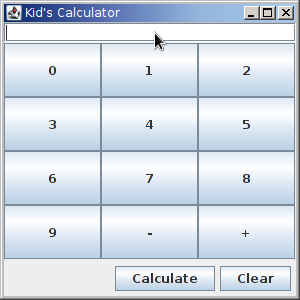
\includegraphics[scale=0.6]{other/calculator.png}
\end{minipage} \hfill

\vspace{-60pt}
\begin{answer}
\begin{lstlisting}[language=java,basicstyle=\scriptsize]
public class KidsCalc extends Application {
    private final static int BUTTON_WIDTH = 80;
    private final static int BUTTON_HEIGHT = 50;
    private final static int MIN_WIDTH = BUTTON_WIDTH*3;

    public void start(Stage primaryStage) throws Exception {
        Scene scene = new Scene(this.makeMainPane());
        primaryStage.setTitle("Kid's Calculator");
        primaryStage.setScene(scene);
        primaryStage.show();
    }

    private Parent makeMainPane() {
        BorderPane bp = new BorderPane();	//BORDER PANE LAYOUT
        bp.setPrefWidth(MIN_WIDTH);
        bp.setTop(makeTopArea()); 		//TOP
        bp.setCenter(makeCenterArea());	//CENTER
        bp.setBottom(makeBottomArea());	//BOTTOM
        return bp;
    }

    private Node makeTopArea(){
        TextField t = new TextField("0");
        t.setEditable(false);
        return t;
    }

    private Node makeCenterArea(){
        FlowPane flow = new FlowPane();
        flow.setMinWidth(MIN_WIDTH);
        
        for(int i = 0; i<10; i++){	// buttons 0 - 9
            Button b = new Button(String.valueOf(i));
            b.setPrefSize(BUTTON_WIDTH,BUTTON_HEIGHT);
            flow.getChildren().add(b);
        }
        
        Button minus = new Button("-"); 
        minus.setPrefSize(BUTTON_WIDTH,BUTTON_HEIGHT);
        flow.getChildren().add(minus);
        Button plus = new Button("+");
        plus.setPrefSize(BUTTON_WIDTH, BUTTON_HEIGHT);
        flow.getChildren().add(plus);
        return flow;
    }

    private Node makeBottomArea(){
        HBox bottom = new HBox(8);				//HBox for bottom row
        bottom.setAlignment(Pos.CENTER_RIGHT);
        Button calculate = new Button("Calculate");	//calculate button
        bottom.getChildren().add(calculate);
        Button clear = new Button("Clear");			//clear button
        bottom.getChildren().add(clear);
        return bottom;
    }
}
\end{lstlisting}
\end{answer}
